%! TEX program = pdflatex

\documentclass[journal]{IEEEtran}
\usepackage[pdftex]{graphicx}
\usepackage[colorlinks=true,urlcolor=blue,citecolor=blue, linkcolor=blue]{hyperref}
\usepackage{url}
\usepackage{siunitx}
\usepackage{multirow}
\usepackage[table,xcdraw]{xcolor}
\hyphenation{op-tical net-works semi-conduc-tor}
\DeclareRobustCommand{\TMCIT}{Tokyo Metropolitan College of Industrial Technology}
\usepackage[whole]{bxcjkjatype}

\begin{document}

\title{RoboCup Rescue Team Description Material \\
 TUPAC}
 \author{Yuichi~Kikuchi,
        Takumi~Komori,
        Tada~Yusuke% <-this % stops a space
\thanks{Yuichi Kikuchi is with the Department
of Information Processing, \TMCIT, TMCIT, e-mail: m14054@g.metro-cit.ac.jp}% <-this % stops a space
\thanks{Takumi Komori is with the same college}%
\thanks{Tada Yusuke is with the same college}%
}
\markboth{RoboCup Rescue TDP Collection}%
{Kikuchi \MakeLowercase{\textit{et al.}}: TUPAC}
\maketitle

\begin{flushleft}
\textbf{Info}\\
\hspace{10pt} Team Name: \hfill TUPAC\\
\hspace{10pt} Team Institution: \hfill Tokyo Metropolitan College of\\
\hfill Industrial Technology\\
\hspace{10pt} Team Leader: \hfill Yusuke Tada\\
\hspace{10pt} Team URL: \hfill % \url{https://moon.edu}
\\
\vspace{5pt}
\hspace{10pt} RoboCup Rescue TDP collection: \\
\hfill \url{http://wiki.robocup.org/Robot_League}
\end{flushleft}

\begin{abstract}
Recently, we have a lot of serious natural disasters.
It is clear that rescue robots are needed to save people's lives.
However, they are difficult to be built, because they have huge actuators which cost a lot.
Very high technologies are also needed to make large hardware and flexible software which have great reliability.
Thus, we developed a simple remote-controlled rescue robot using the techniques we learned form RoboCup Junior.
This paper describes about hardware and software of our robot, ``TUPAC''.
\end{abstract}

\begin{IEEEkeywords}
RoboCup Rescue, Team Description Paper. % TODO: add up to 3 keywords
\end{IEEEkeywords}

\IEEEpeerreviewmaketitle

\section{Introduction}
\IEEEPARstart{O}{ur} team consists of two students of \TMCIT.
This is the first time we participate in the RoboCup Rescue Rapid Manufactured League.
However, we have competed in RoboCup Junior for two years.
Kikuchi - the leader of our team - ranked 5th in Rescue A Challenge of RoboCup Junior 2015 Japan Open.
Komori - another member of the team - ranked 5th in Soccer Challenge Light Weight League of RoboCup Junior 2015 Hefei World Competitions.
We were not in the same team in 2015, and we started up a new team in 2016 together.
We merged our knowledges learned from both Rescue and Soccer Challenge.
Because of the lack of experiences, we could not win any titles in 2016, but we found what the problem was and how to solve them.

\section{System Description}
\begin{figure}[!t]
    \centering
    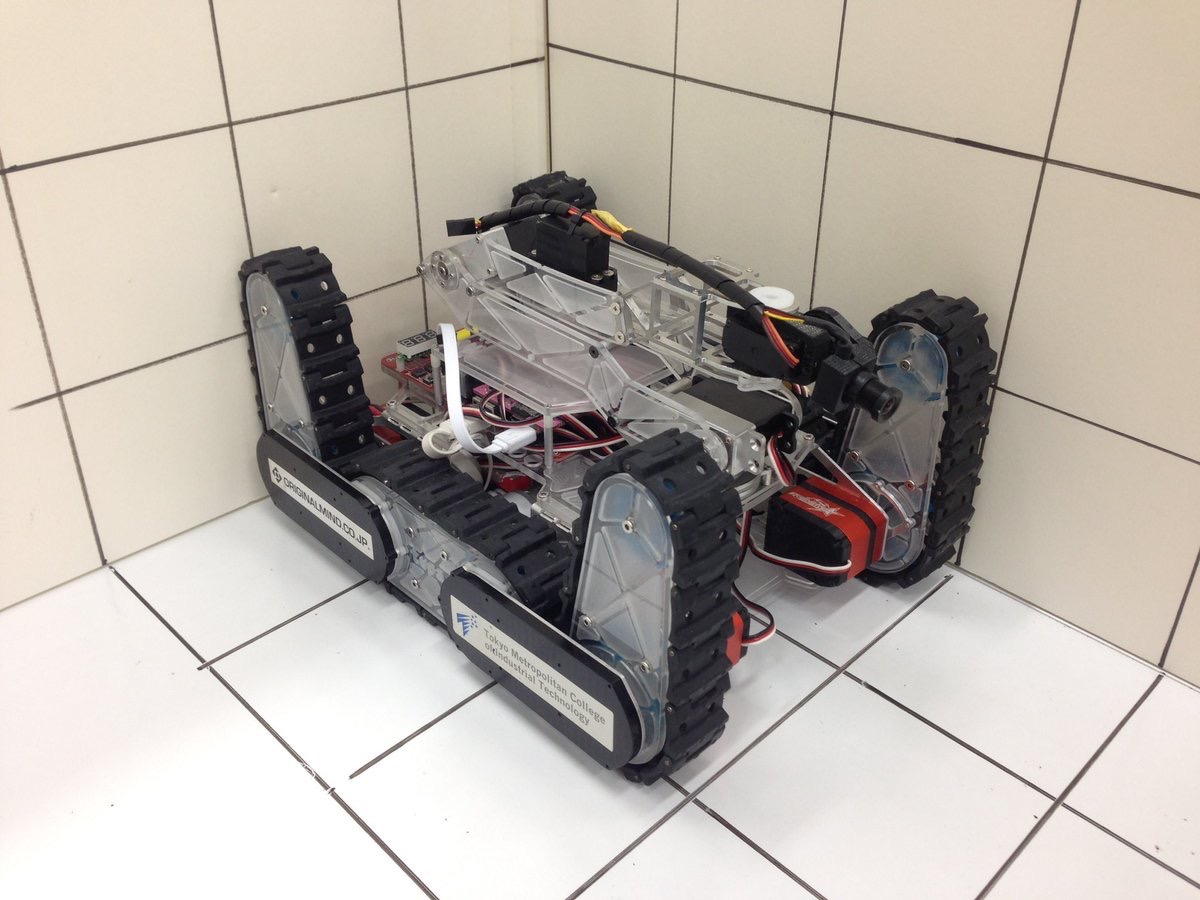
\includegraphics[width=0.45\textwidth]{robot.jpg}
    \caption{TUPAC} \label{fig:robot}
\end{figure}
In this section, we describe more details of the ``TUPAC'' on separate views.
Figure \ref{fig:robot} shows the robot.

\subsection{Mechanic}
It was difficult to create a robot which is controlled by a human unlike RoboCup Junior, but the size is as small as Junior ones.
Especially flipper arm should be within \(\SI{30}{\cm} \times \SI{30}{\cm}\).
The field also makes it difficult.
It is flat in Junior, but there are many stairs in it.

\subsubsection{Locomotion}
The robot has two continuous tracks driven by two DC motors and four independent flipper arm controlled by four servo motors to move.
Flipper arms can tilt \SI{\pm60}{\degree} against the horizontal and can be driven with continuous tracks at the same time.
The robot can run on rough terrain with high stairs by controlling four flipper arms unlike conventional wheeled system.

% \subsubsection{Shape}
% The robot is designed based on the robot we created for RoboCup Junior.
% Two continuous track is placed in left and right side.
% Four flipper arm is placed in forward and backward side.
% When flipper arm is lifted up, the robot takes square shape.
% It protects components from debris while moving.

% A camera is placed in forward side.
% It is not supposed to turn around.
% We should control the robot turn around to view the back side.

% There is no tires or crawlers to prevent the robot from falling down except for flipper arm.
% When it occurs, flipper arm raise the robot up if possible.

% \subsubsection{Speed}
% Motors are Tamiya 380 which is commonly used in RoboCup Junior.
% Planetary gears are used to convey torques and prevent it from aging.
% The robot moves slow basically, and accelerates for stairs.
% Gears make it decelerate and improve torques.

% \subsubsection{Size}
% There is no specification for the size of robots.
% We designed the robot for the field which size is \(\SI{30}{\cm} \times \SI{30}{\cm}\).
% Its size is within \(\SI{25}{\cm} \times \SI{25}{\cm}\) when the flipper arm is lifted up to make turning around without moving possible.

% The body is made of \SI{4}{\mm} polycarbonate.
% It has resistance against damage from impact and fire and is easy to manufacture.

% \begin{figure}[!t]
%     \centering
%     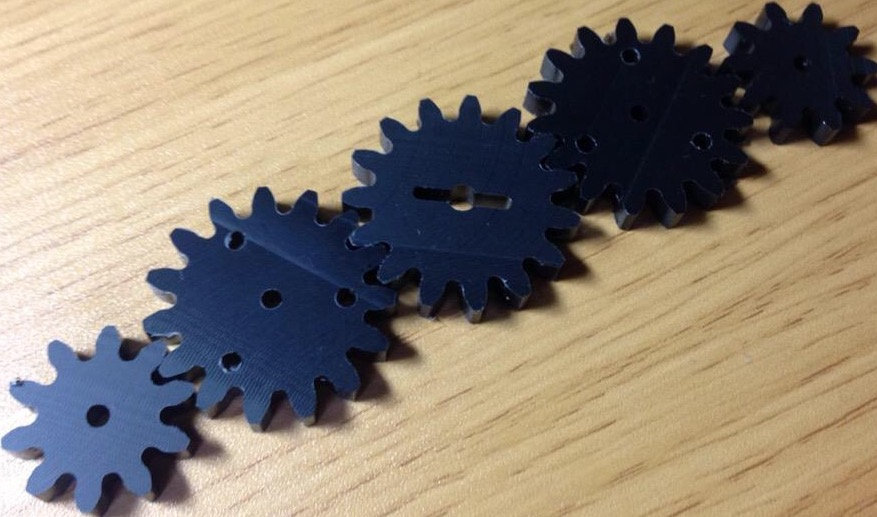
\includegraphics[width=0.45\textwidth]{gear.jpg}
%     \caption{Gear} \label{fig:gear}
% \end{figure}
% Figure \ref{fig:gear} shows the gears used to convey driving force.
% They are made of POM.
% It has slidability and resistance against damage from abrasion.
% It can be used for long time continuously.

% \begin{figure}[!t]
%     \centering
%     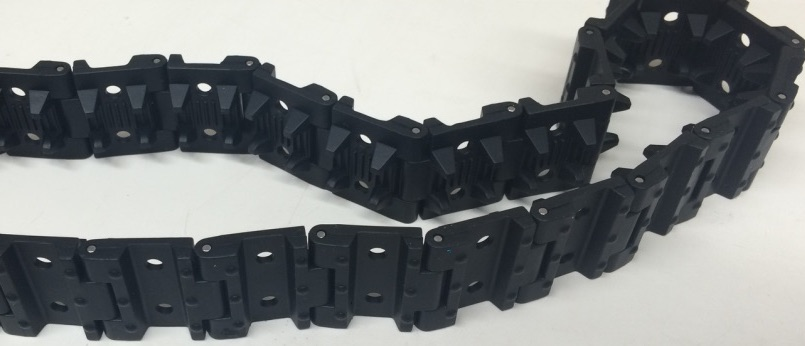
\includegraphics[width=0.45\textwidth]{crawler.jpg}
%     \caption{Crawler} \label{fig:crawler}
% \end{figure}
% Figure \ref{fig:crawler} shows the crawler used for both of main and sub ones.
% It is made of rubber which makes friction on field.
% The friction makes it easy to move.
% Projections on crawler helps it to climb stairs.

% \subsubsection{Manufacturability}
% The hardware can be built within low costs.
% The materials, crawler, gears can be purchased.
% Polycarbonate was manufactured with CNC milling machine.
% Shafts and other components are manufactured by hand.

\subsection{Power}
The robot is equipped with 2-cells \SI{7.4}{\V} \SI{2200}{mAh} lithium-polymer battery as the source of power and can run about 20 minutes with charging once.
Voltage from the battery is delivered to two DC motors, nine flippers, servo motors for manipulators directly.
It is also delivered to a microcontroller and a Wi-Fi router through a DC-DC converter.
Figure \ref{fig:system} shows the system diagram.
\begin{figure}[!t]
    \centering
    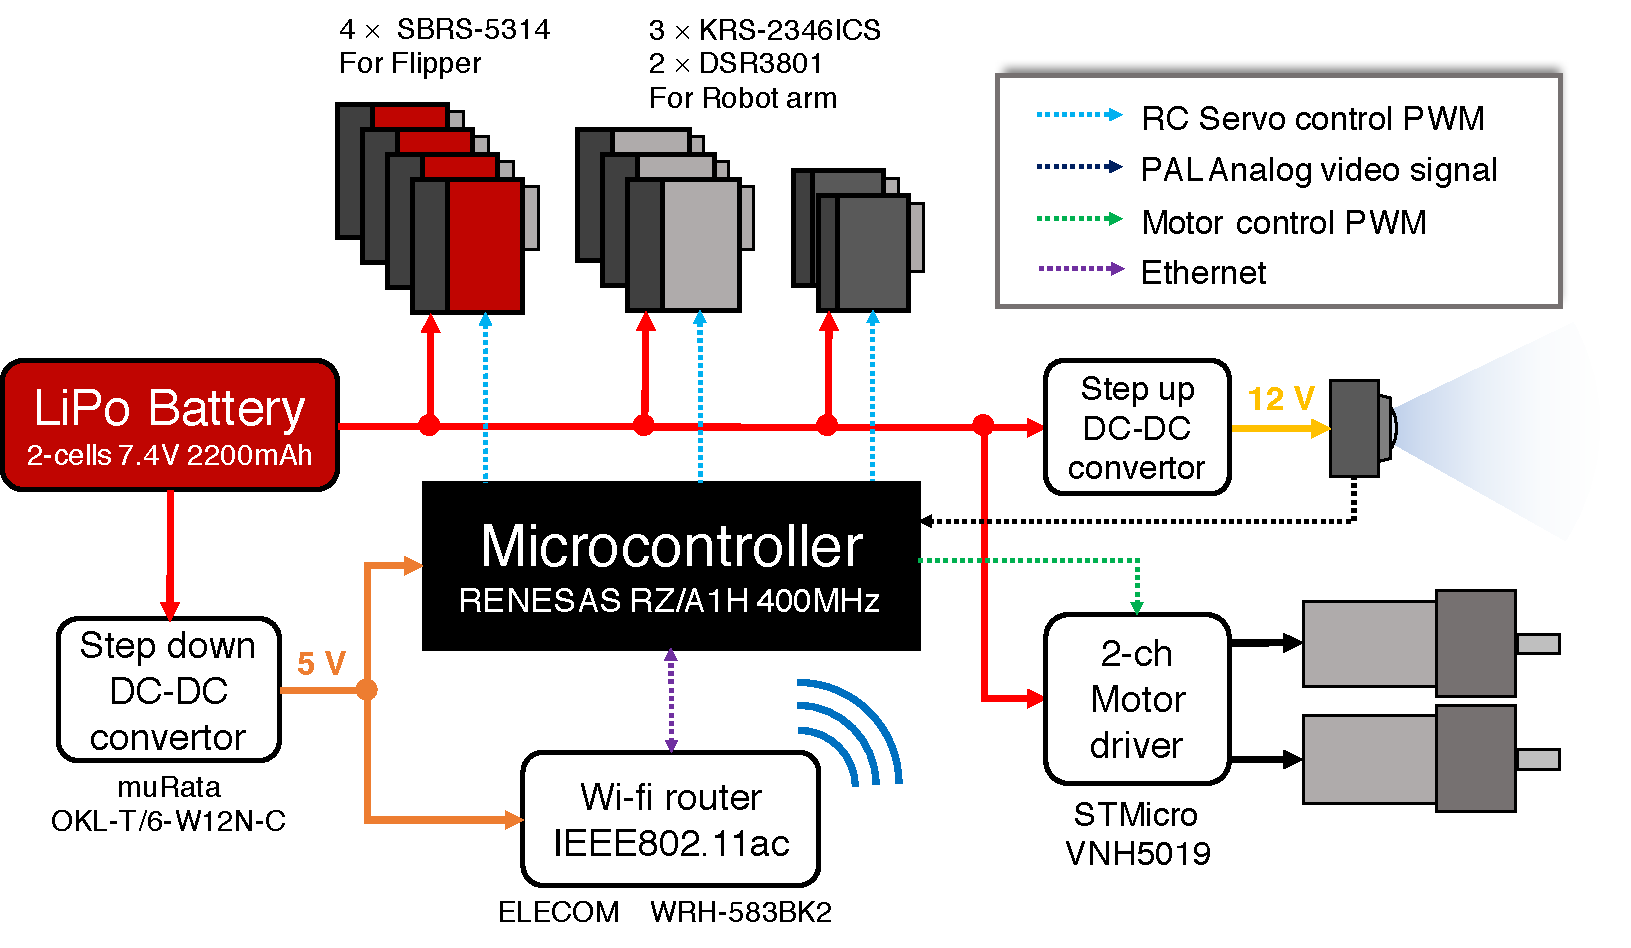
\includegraphics[width=0.45\textwidth]{System_diagram.pdf}
    \caption{System diagram} \label{fig:system}
\end{figure}

\subsection{Electronic circuit}
``TUPAC'' has one electronic circuit board.
It consists of following components.
\begin{itemize}
    \item Renesas GR-Peach \\
    This microcontroller board carries an MCU, Reneas RZ/A1H.
    It has Ethernet connector, hardware NTSC/PAL decoder, hardware JPEG encoder, several PWM timers, and many GPIOs.
    These capabilities are enough to control entire robot, and it can handle all of them because of its very high CPU frequency (at \SI{400}{\MHz}).
    Also, it is arm mbed enabled. % TODO: 正式なARMの表記
    This means GR-Peach can be controlled by well-abstracted C++ APIs.
    We developed software quickly thanks to the wonderful library.
    \item VNH5019 \\
    This brushed DC motor driver appears twice in the main board, one for the left, another for the right motor.
    It can drive \(\pm\)\SI{30}{\A} continuously, and has various protection features such as short circuit, current, and temperature.
    It has enough function to drive Tamiya 380 smoothly and safely.
    \item OKL-T/6-W12N-C \\
    This DC-DC converter generates stabilized voltage at \SI{5}{\V}.
    It is mainly used for operating the portable Wi-Fi router and the CMOS camera.
    This converter can supply up to \SI{6}{\A}. % TODO: 6Aだっけ
    So we power all the \SI{5}{\V} devices by this converter without worry.
    \item Connectors \\
    The board can connect  up to 10 servo motors.
    These motors can be controlled by PWM signals from GR-Peach.
    There is also CMOS camera connector to let GR-Peach receive NTSC/PAL TV signal from the camera.
\end{itemize}

\subsection{Manipulation}
The robot is equipped with a 5-DoF robot arm.
The length of link of robot arm is \SI{225}{\mm} and each freedom has \SI{\pm60}{\degree} range of movement.
This robot arm is designed to be able to see not only the front of the robot but also right and left side, ground, ceiling, and back side.

\subsection{Sensors}
Our robot is not equipped with any sensors.
But in this competition, an issue that the operator cannot tell the situation of the robot such as inclination, direction, and so on had occurred.
We are considering using IMU to detect angles as a solution to this issue.

\subsection{Software}
In this section, we describe the software of ``TUPAC''.
\subsubsection{Communication Protocol}
The robot and PC communicate each other through the original protocol we designed.
It is named RDTP (Robot Data Transfer Protocol), and it is on the application layer of the Internet protocol suite.
\begin{table}[!t]
\centering
\caption{Structure of RDTP Packet} \label{tbl:rdtp}
\begin{tabular}{
>{\columncolor[HTML]{C0C0C0}}c |cl}
Bit Offset & \cellcolor[HTML]{C0C0C0}0$\sim$7 & \multicolumn{1}{c}{\cellcolor[HTML]{C0C0C0}8$\sim$15} \\
0          & \multicolumn{2}{c}{Header}                                                               \\
16         & \cellcolor[HTML]{FFCCC9}Value0   & \cellcolor[HTML]{FFCCC9}Value1                        \\
32         & Value2                           & Value3                                                \\
64         & \multicolumn{2}{c}{\cellcolor[HTML]{FFCCC9}...}                                         
\end{tabular}
\end{table}

Table \ref{tbl:rdtp} shows the structure of an RDTP packet.
First 2 bytes contain a header.
Following bytes are variable-length.
They contain individual component values in order.

\begin{table}[!t]
\centering
\caption{RDTP Packet Header} \label{tbl:rdtpheader}
\begin{tabular}{c|cc}
\rowcolor[HTML]{C0C0C0} 
Bit                                & Name         & Value               \\ \hline
\cellcolor[HTML]{C0C0C0}0          & LeftMotor    & Motor power         \\
\rowcolor[HTML]{FFCCC9} 
\cellcolor[HTML]{C0C0C0}1          & RightMotor   & Motor power         \\
\cellcolor[HTML]{C0C0C0}2          & Servo0       & Servo angle         \\
\rowcolor[HTML]{FFCCC9} 
\cellcolor[HTML]{C0C0C0}3          & Servo1       & Servo angle         \\
\cellcolor[HTML]{C0C0C0}$\vdots$   & $\vdots$     & $\vdots$            \\
\rowcolor[HTML]{FFCCC9} 
\cellcolor[HTML]{C0C0C0}11         & Servo9       & Servo angle         \\
\cellcolor[HTML]{C0C0C0}12         & EnableServo  & Servo \# to enable  \\
\rowcolor[HTML]{FFCCC9} 
\cellcolor[HTML]{C0C0C0}13         & DisableServo & Servo \# to disable \\
\cellcolor[HTML]{C0C0C0}14$\sim$17 & \multicolumn{2}{c}{Reserved}      
\end{tabular}
\end{table}

\begin{table}[!t]
\centering
\caption{Example of an RDTP Packet} \label{tbl:rdtpex}
\begin{tabular}{c|cc}
\rowcolor[HTML]{C0C0C0} 
Bits                       & 0            & 1           \\ \hline
\cellcolor[HTML]{C0C0C0}0  & \multicolumn{2}{c}{0x1023} \\
\rowcolor[HTML]{FFCCC9} 
\cellcolor[HTML]{C0C0C0}16 & 42           & -24         \\
\cellcolor[HTML]{C0C0C0}32 & 200          & 7          
\end{tabular}
\end{table}

Table \ref{tbl:rdtpheader} shows the structure of the header in an RDTP packet.
Each bit has different components to control.
To assign zero to all bits has special meaning.
It indicates there is a command instead of values.
Command will be in Value0 field as an ASCII character.
Command `V' means ``Start Video'', `v' means ``Stop Video''.

Table \ref{tbl:rdtpex} shows an example of one complete RDTP Packet.
It means as follows
\begin{itemize}
    \item Drive left motor forward as power of 42/127.
    \item Drive right motor backward as power of 24/128.
    \item Set servo motor number 3 angle 200/255.
    \item Enable servo motor number 7.
\end{itemize}

RDTP packet is delivered in UDP packet.
In robot controlling, seamlessness is more important than correctness.
Therefore, UDP packet is more suitable than TCP packet.
Packets are send in \SI{10}{\ms} period.
This is 5 times faster than general radio controller, and it realizes the smooth controlling.

\subsubsection{Robot}
The program is written in C++14.
It uses ARM mbed library (we contributed a little) for the low-level implementations.
Figure \ref{fig:class_robot} shows the class diagram.
\begin{figure*}
    \centering
    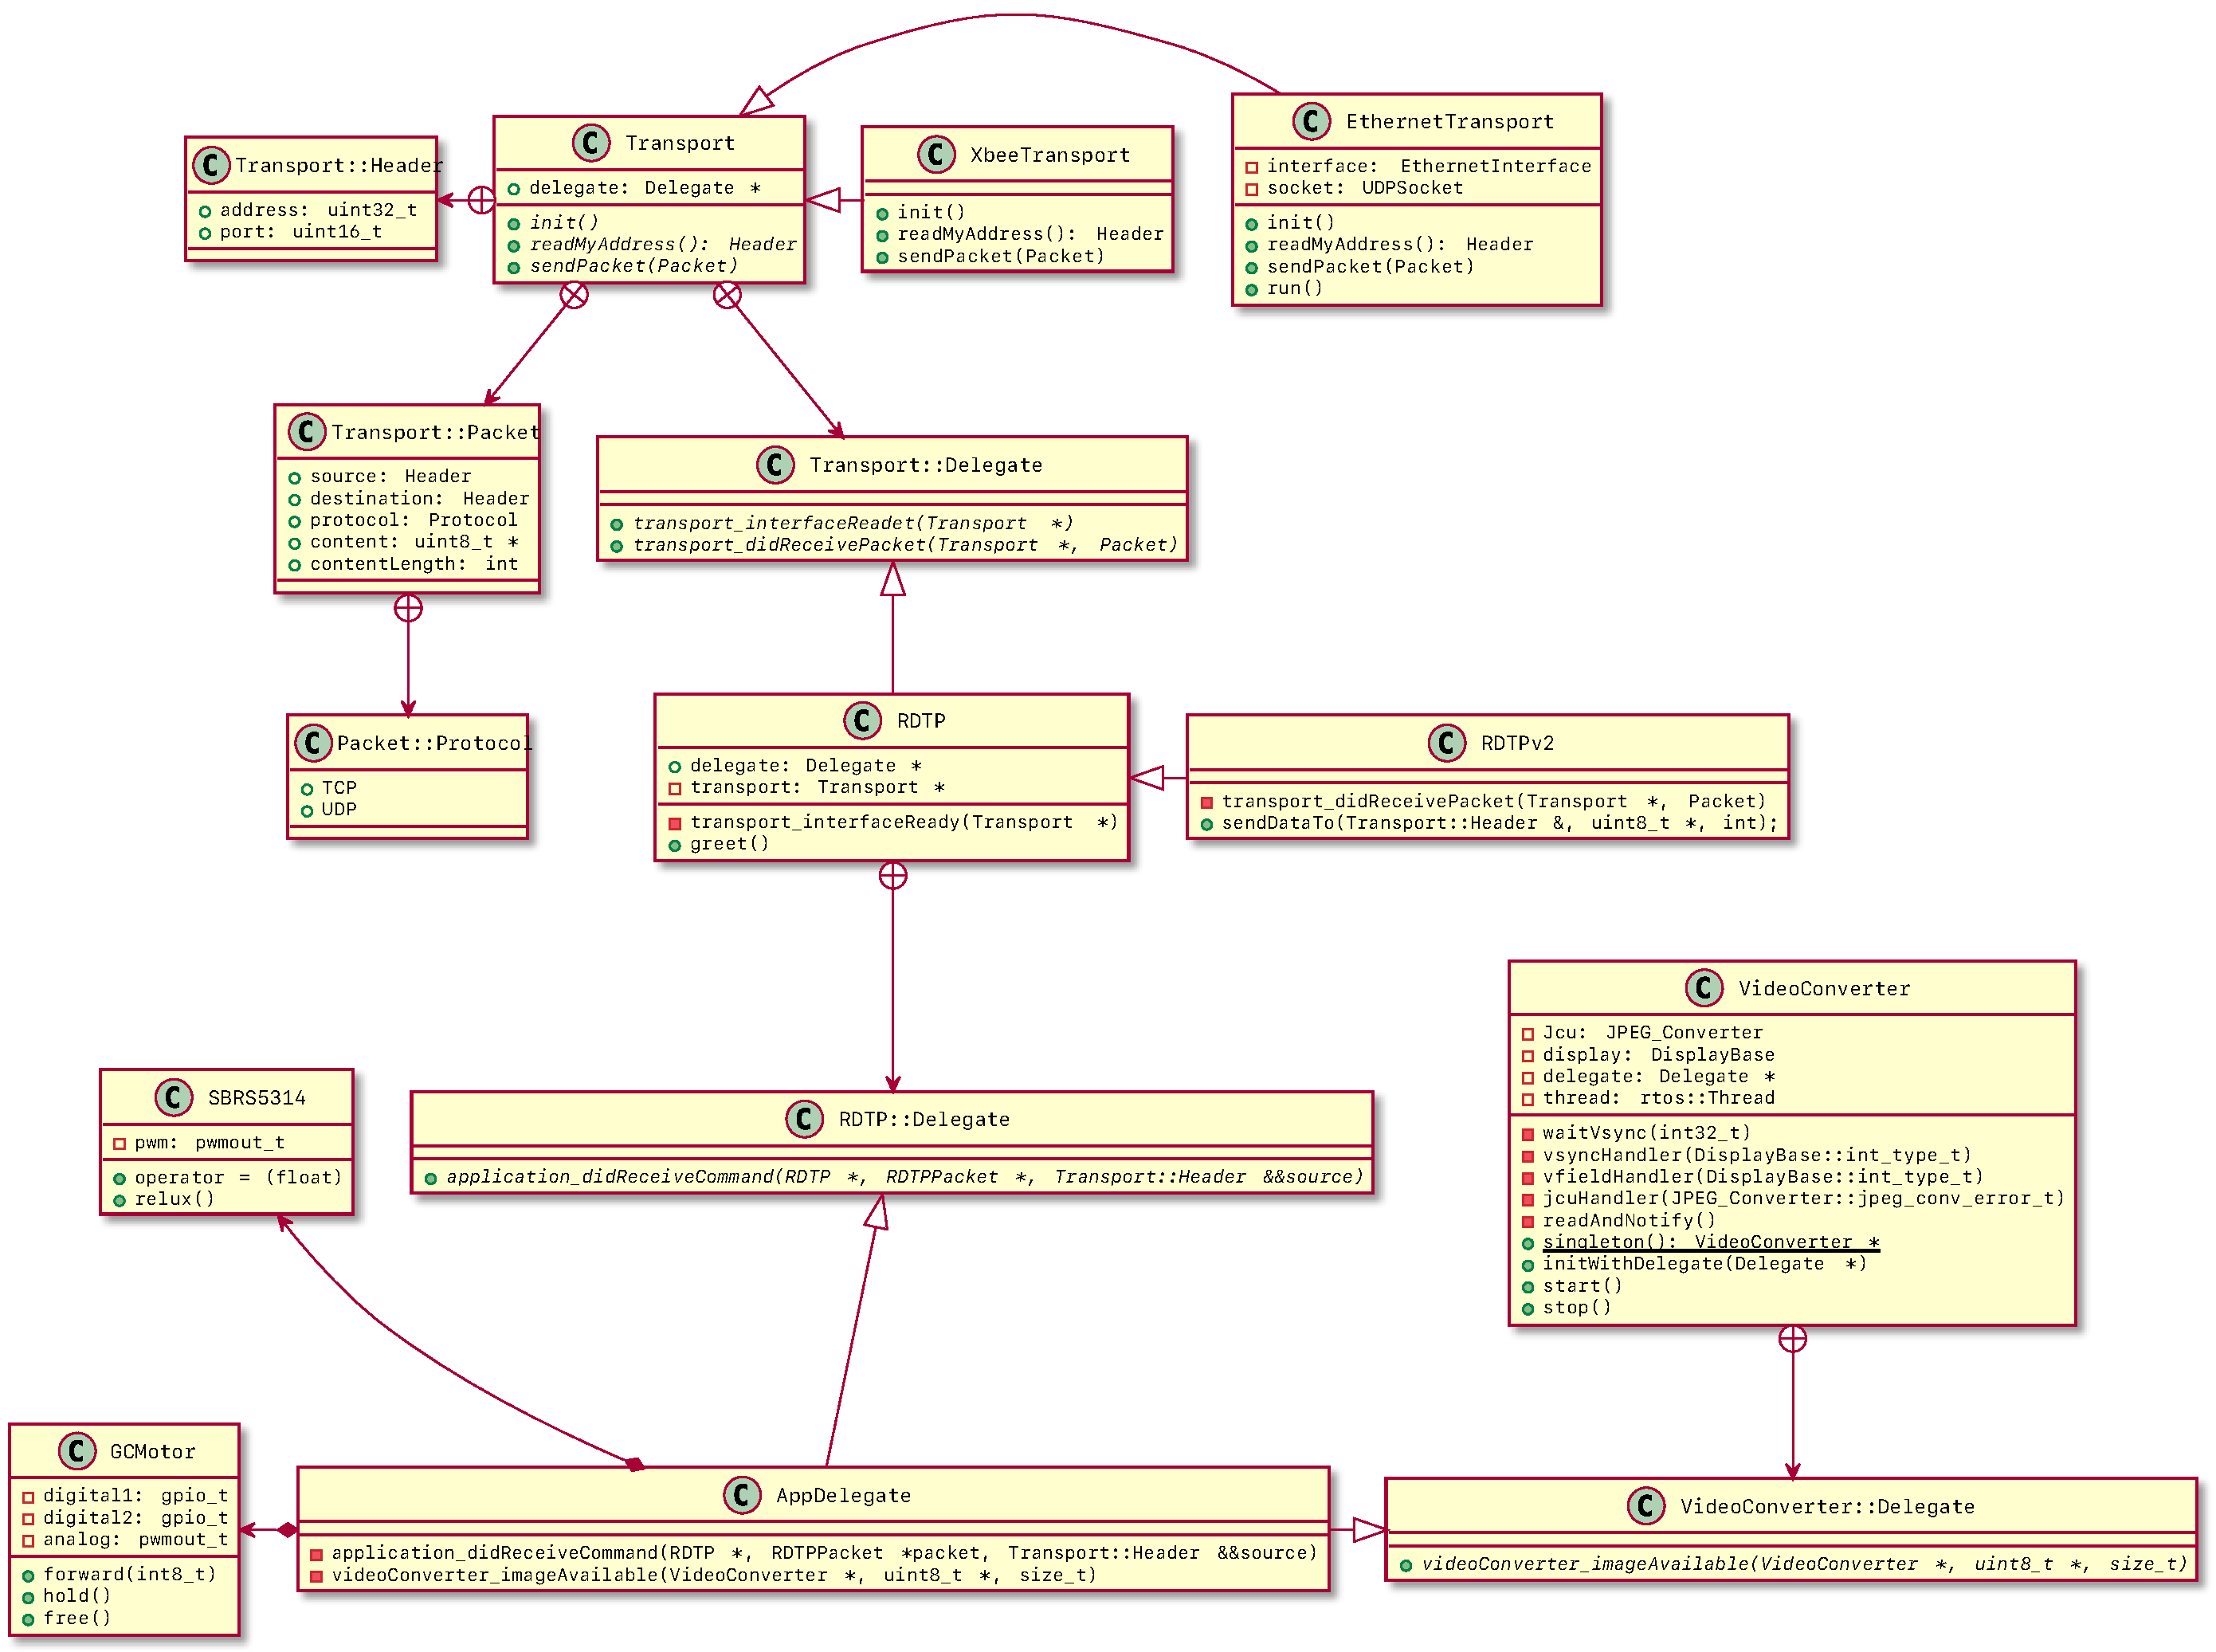
\includegraphics[width=1.0\textwidth]{robotClass.pdf}
    \caption{Class diagram of robot} \label{fig:class_robot}
\end{figure*}

First, it sends an UDP broadcast packet so the host PC can know the IP address of the robot.
After that, it waits for an RDTP packet and process it.
Figure \ref{fig:transport} shows the activity diagram of processing loop.
This method, ``EthernetTransport::run()'' is called from ``main()'', is the main loop of this program.
\begin{figure*}
    \centering
    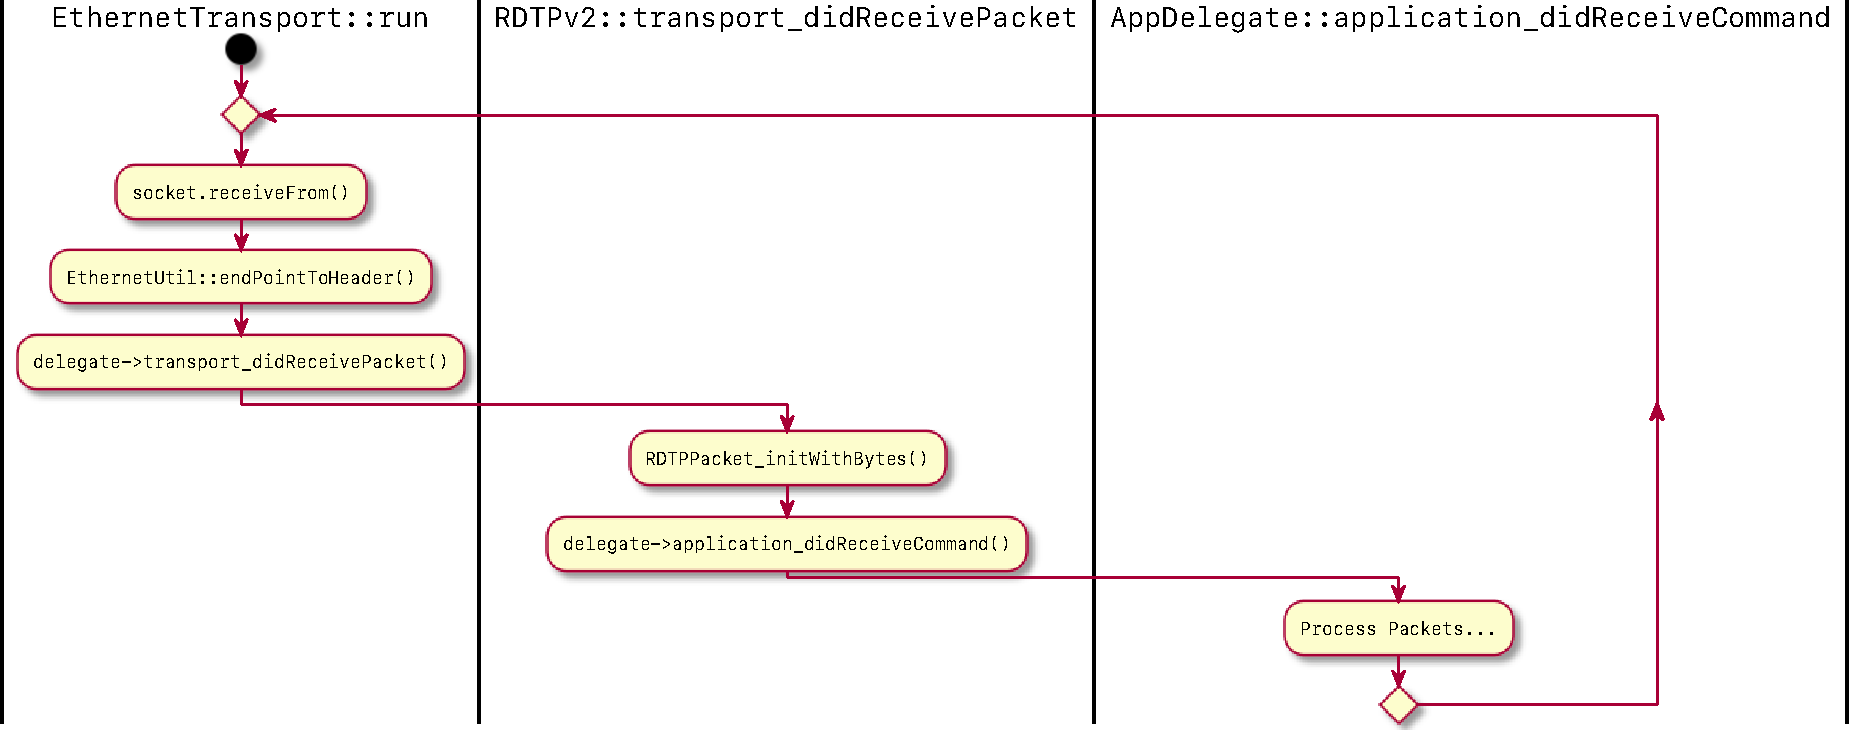
\includegraphics[width=1.0\textwidth]{transport.pdf}
    \caption{Activity diagram of EthernetTransport::run()} \label{fig:transport}
\end{figure*}

When a packet is arrived, ``AppDelegate::application\_didRe-\\ceiveCommand()'' will be invoked to process it.
Figure \ref{fig:appdelegate} shows the activity diagram of that method.
This loop extracts every single components from the packet, and call a dedicated instance to control actuators or a video converter.
\begin{figure*}
    \centering
    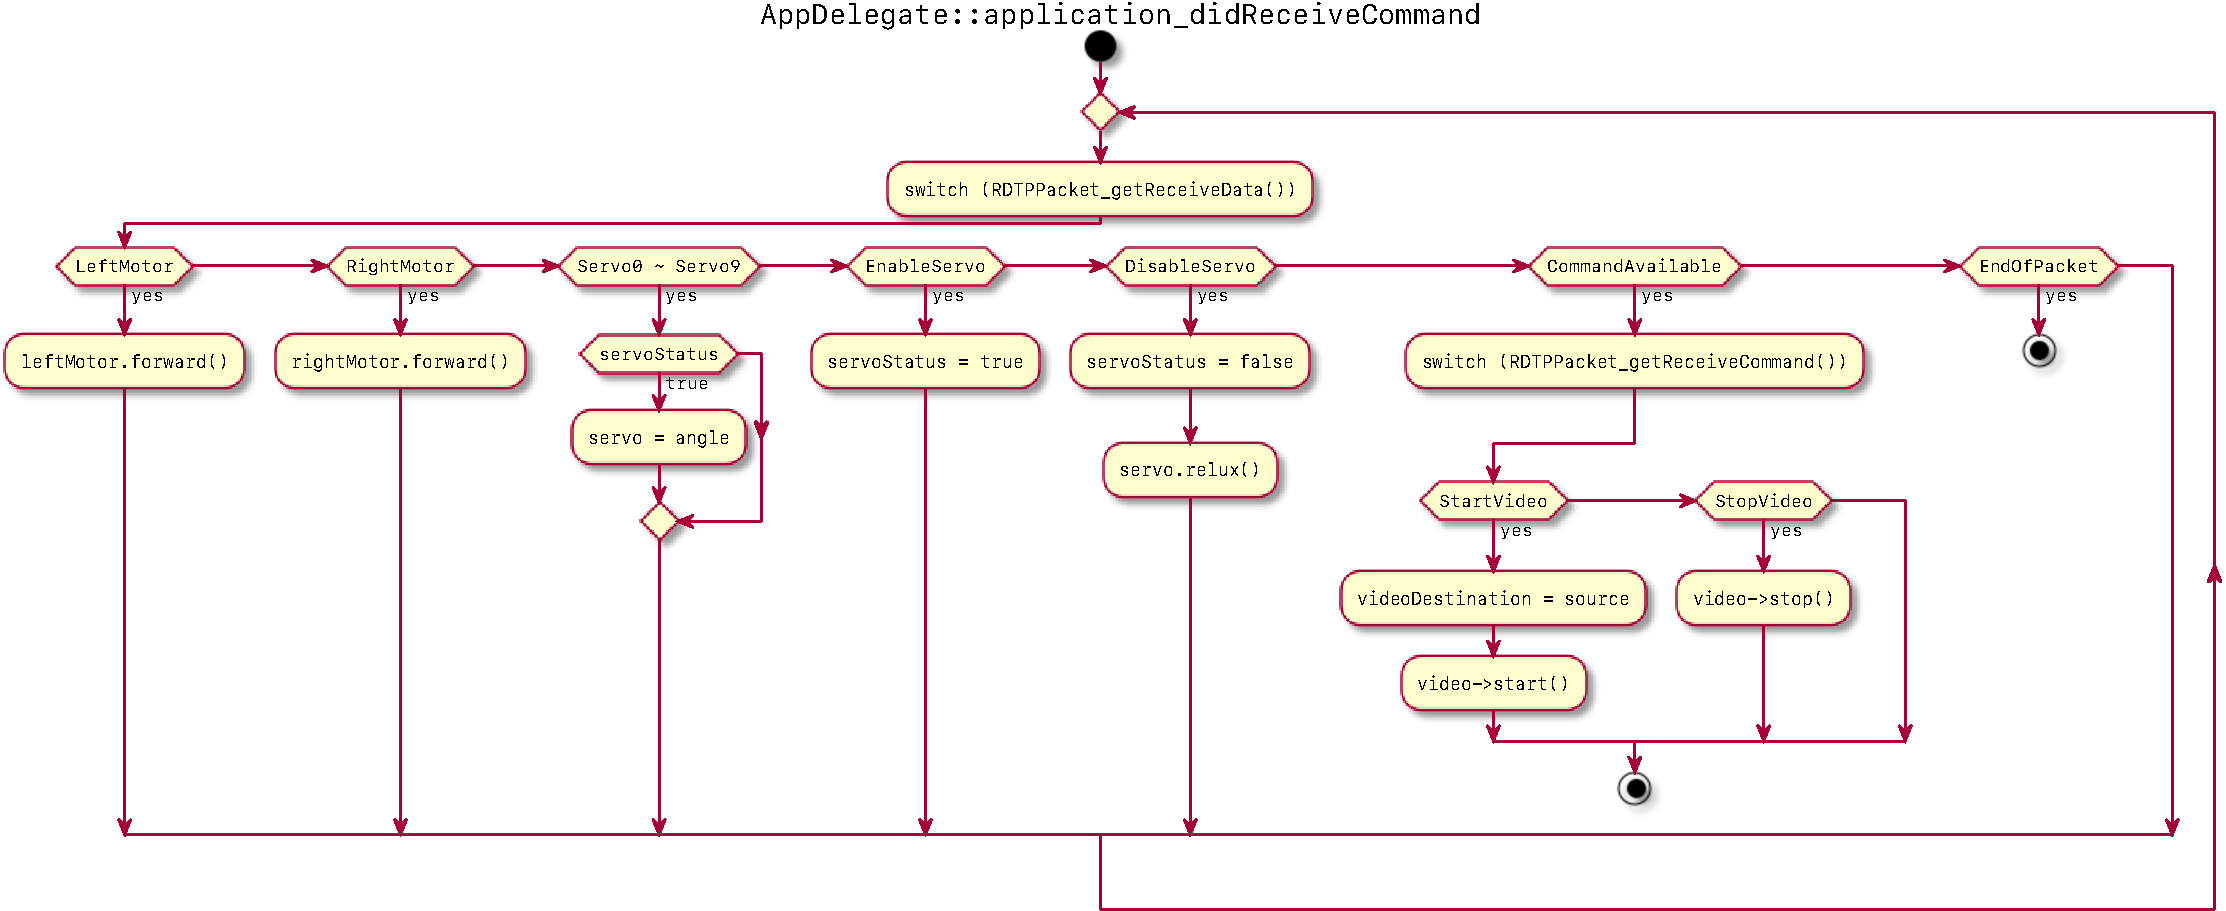
\includegraphics[width=1.0\textwidth]{appdelegate_packet.pdf}
    \caption{Activity diagram of AppDelegate::Packet()} \label{fig:appdelegate}
\end{figure*}

Figure \ref{fig:videoConverter} shows the sequence diagram which describes how the video converter works.
First, it is launched by AppDelegate in accordance with the request ``StartVideo'' in an RDTP packet.
Then it invokes ``DisplayBase::Video\_Start()'' to start hardware NTSC/PAL signal processing.
When ``vfield'' occurs, it means we captured a new frame.
VideoConverter calls JPEG\_Converter immediately to compress raw frame data into a JPEG image.
After conversion finished, interrupt is occurred and VideoConverter handles it.
The handler sets a flag to wake reading thread up, and it tell AppDelegate that a new frame is available.
AppDelegate simply sends that data to the host PC.
\begin{figure*}
    \centering
    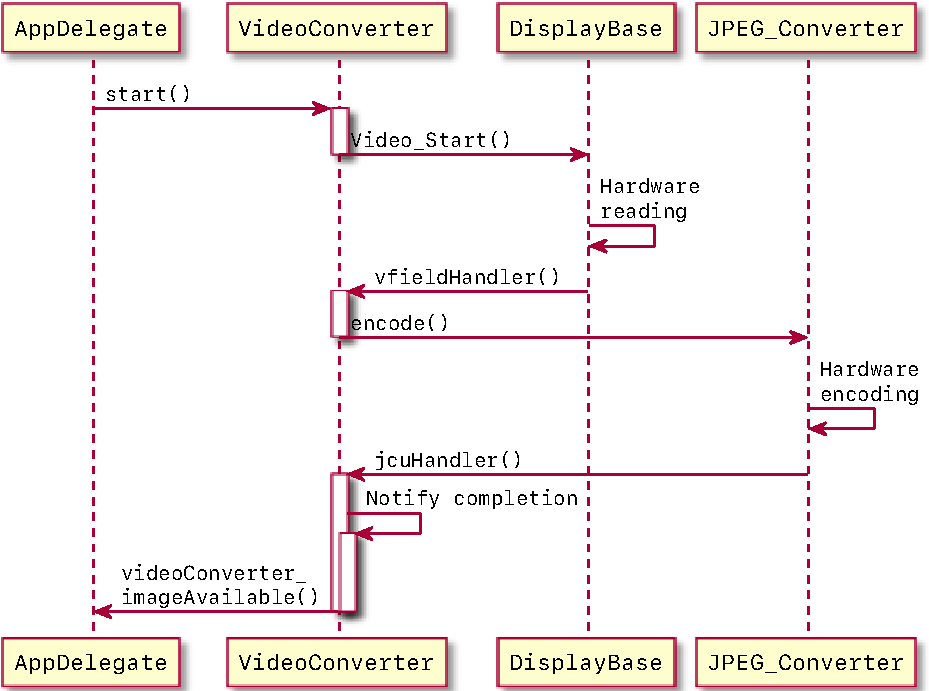
\includegraphics{videoConverter.pdf}
    \caption{Sequence diagram of VideoConverter} \label{fig:videoConverter}
\end{figure*}

As you can see in the diagrams, the program is designed to reduce CPU usage.
Processing video image and Internet packet is a heavy load.
Thus, we should process them through the hardware.
It makes small single core \SI{400}{\MHz} low power CPU be able to control the entire system.
Neither Raspberry Pi nor NUC is needed.
So the circuit and battery will be small and running time will be long.

\subsubsection{Controller}
The program is written in Objective-C 2.0 .
First, it waits for the UDP broadcast packet from the robot.
As described previously, the host PC can know the IP address of the robot through this packet.
After that, it observes the gamepad and stores current status, and send them to the robot in every \SI{10}{\ms}.

Figure \ref{fig:class_controller} shows the class diagram.
It is simpler than the robot thanks to the open-source libraries, macOS runtimes, and especially the flexibility of Objective-C.
\begin{figure*}
    \centering
    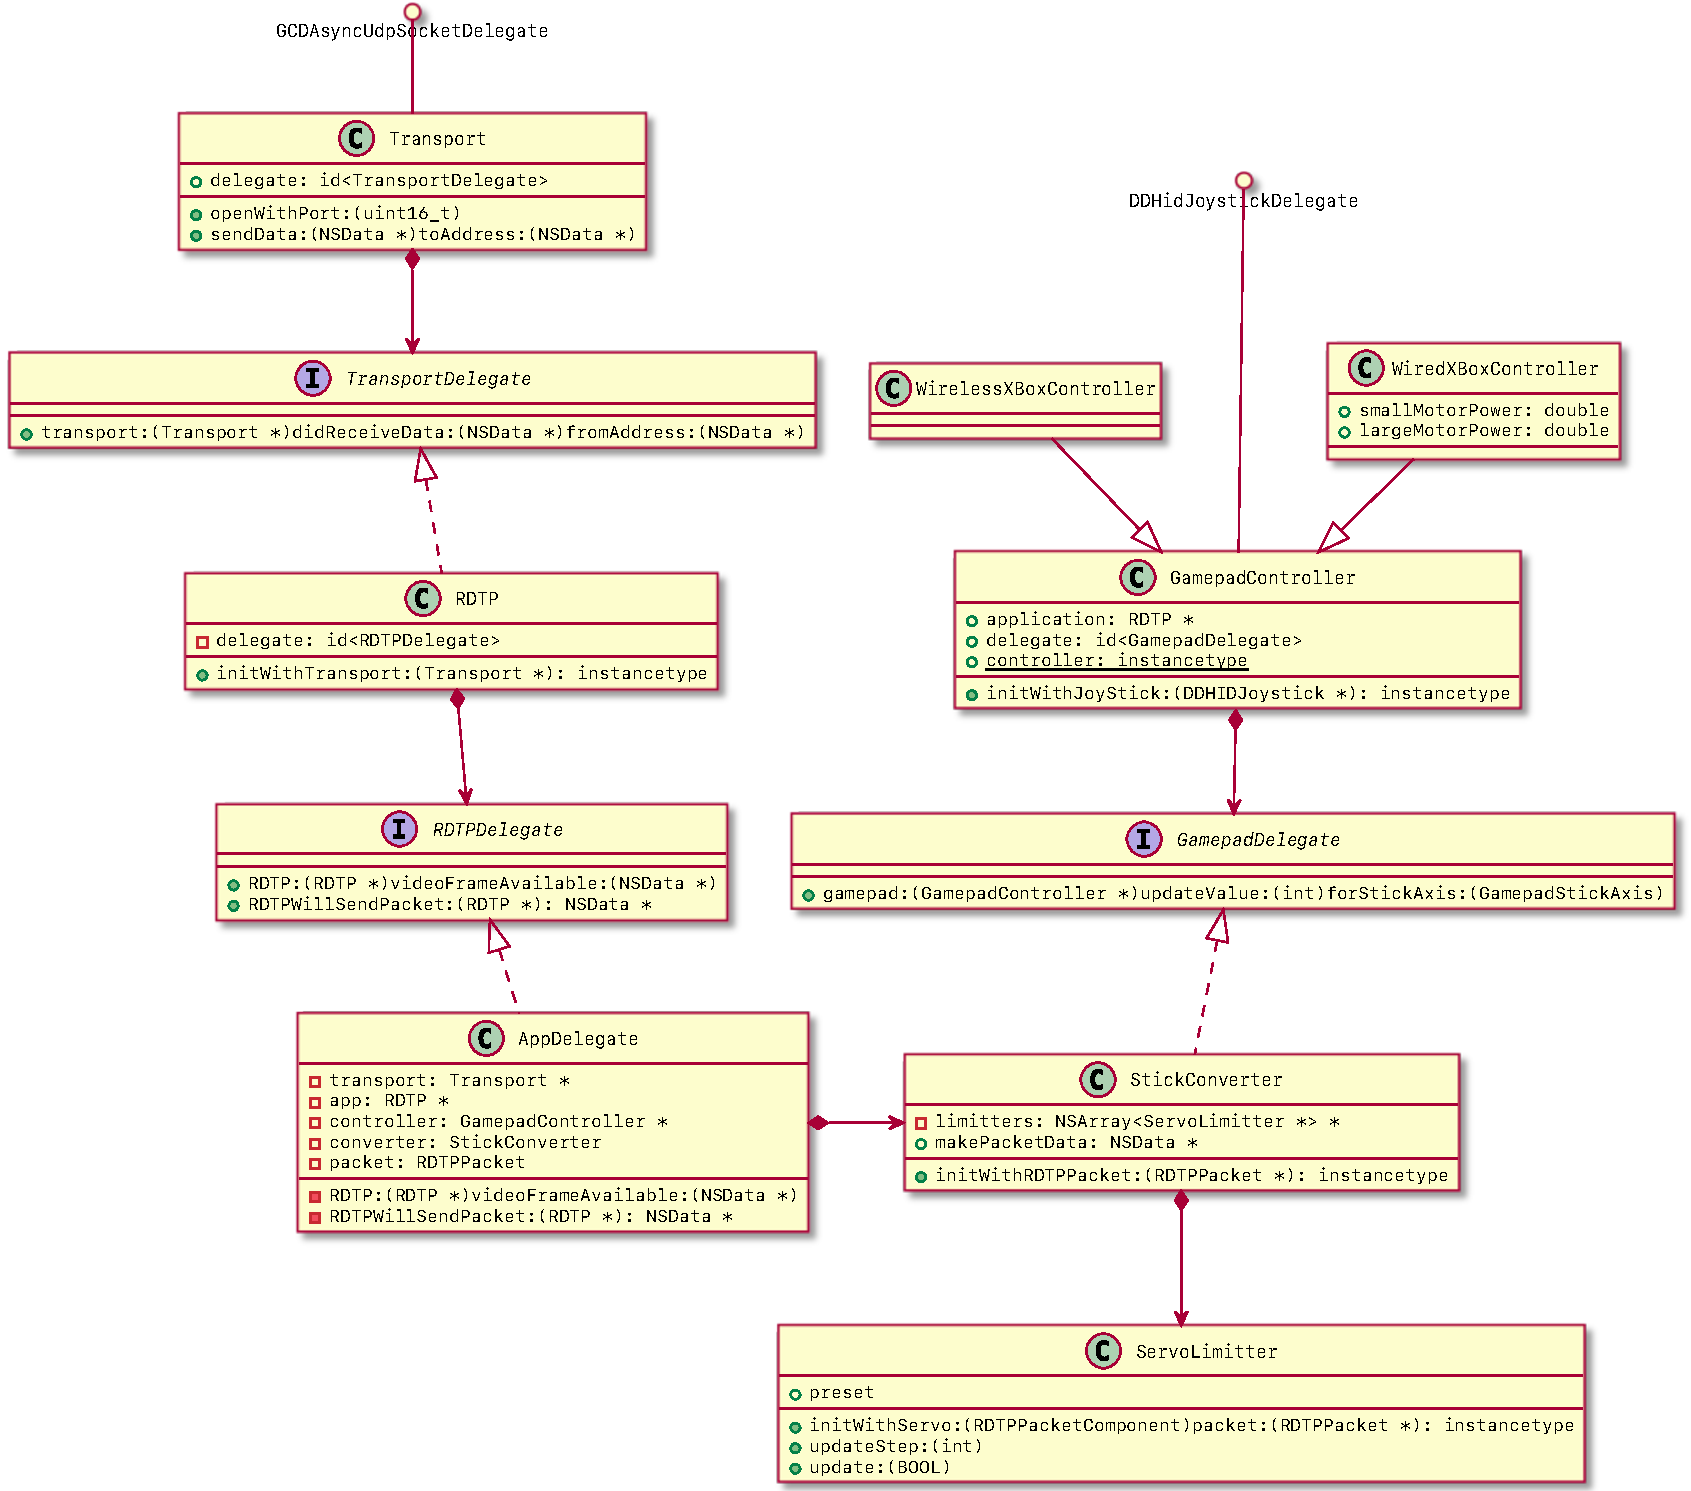
\includegraphics[width=1.0\textwidth]{controllerClass.pdf}
    \caption{Class diagram of controller} \label{fig:class_controller}
\end{figure*}
It uses three open-source libraries.
CocoaAsyncSocket is used for sending and receiving UDP packets.
DDHIDLib is used for observing a gamepad.
Aspects is used for aspect-oriented programming (AOP).

The classes are connected not only with delegates unlike the program on the robot.
When the robot is located, a notification is delivered by RDTP and any class can notice it.
RDTPv2 uses this to start \SI{10}{\ms} timer, and AppDelegate uses this to notify the successful connection to an operator.
AppDelegate also uses AOP techniques to show current gamepad status to an operator.
These informations is normally handled by RDTPv2's instance method updateValue:forStickAxis:.
AppDelegate hooks this selector and get these informations without any modification of RDTPv2.

\subsection{Communication}
The robot carries WRH-583RD2-S portable Wi-Fi router.
It supports IEEE 802.11 ac/n/a/b/g.
We can choose a bandwidth by crowdedness or the amount of physical barriers.

\subsection{Human-Robot Interface}
\begin{figure}[!t]
    \centering
    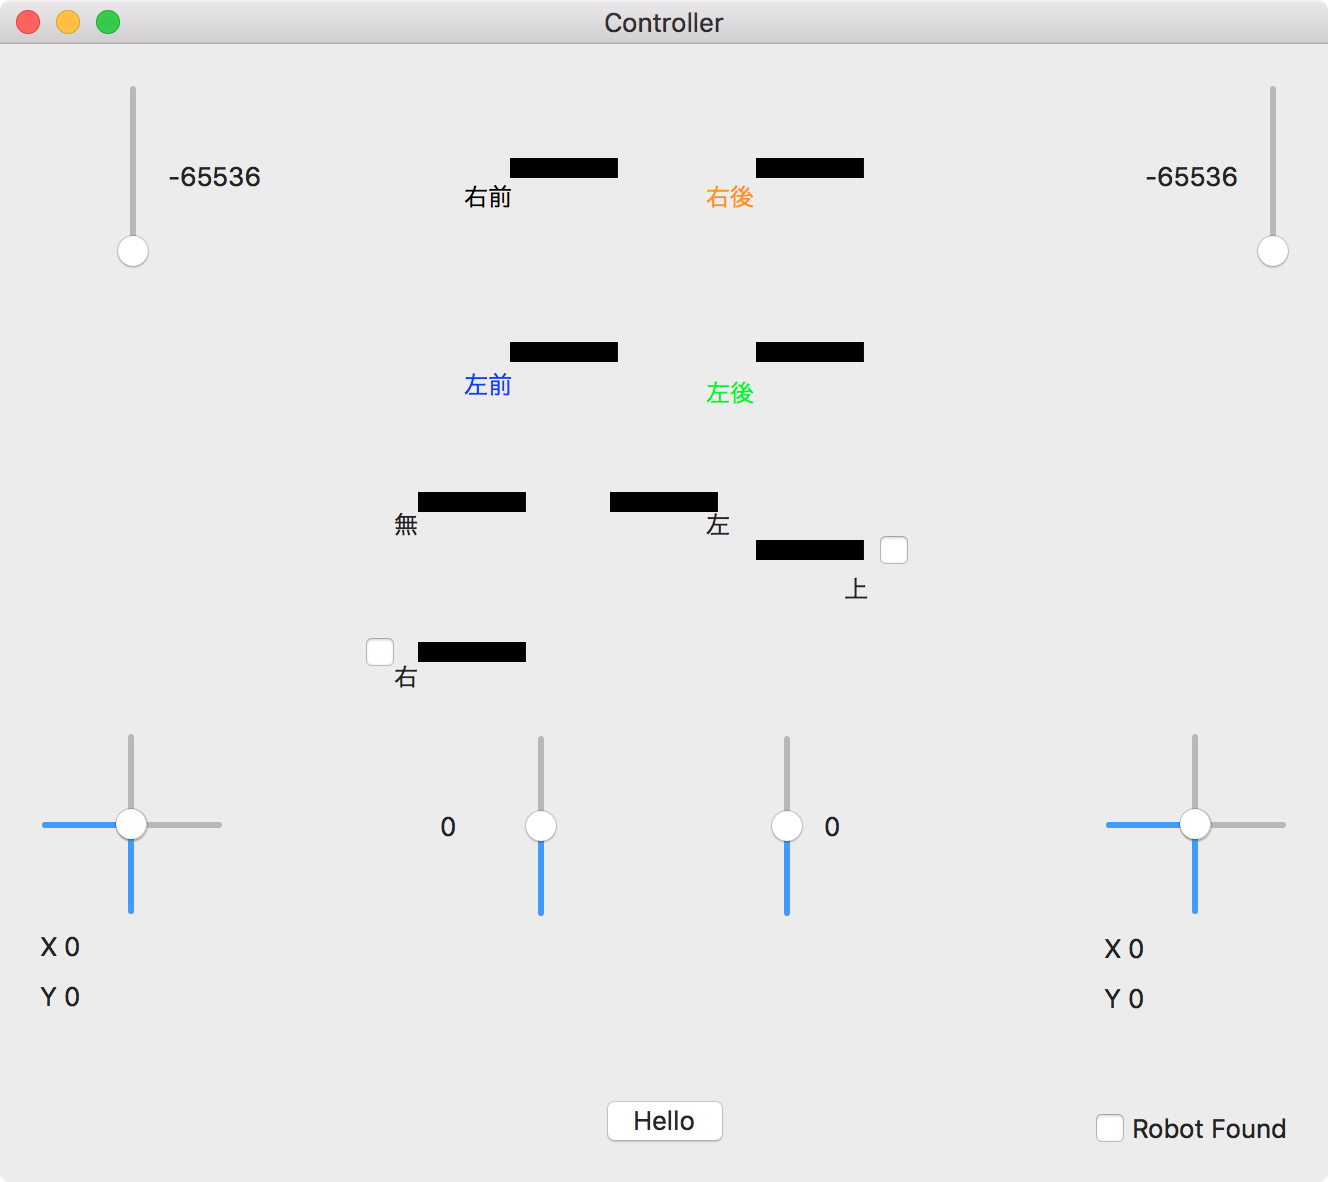
\includegraphics[width=0.45\textwidth]{controller.png}
    \caption{Host application} \label{fig:controller_app}
\end{figure}
Figure \ref{fig:controller_app} shows the interface of the host application.
It shows operators following information.
\begin{itemize}
    \item Stick axis of the gamepad
    \item LR trigger levels of the gamepad
    \item Arm angles with their button configurations
    \item Enable/Disable states of servo motors of the arm
    \item Flipper angles with their button configurations
    \item Whether the robot is found or not
\end{itemize}

\begin{figure}[!t]
    \centering
    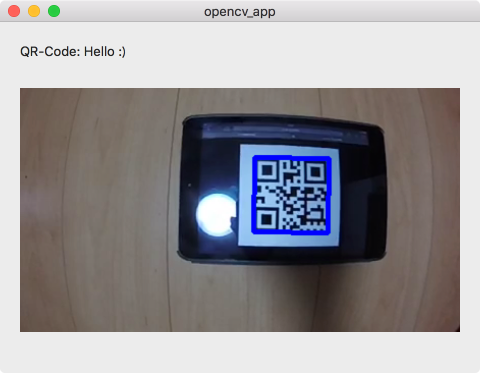
\includegraphics[width=0.45\textwidth]{camera.png}
    \caption{Camera application} \label{fig:camera}
\end{figure}
Figure \ref{fig:camera} shows the camera application.
This captures video streaming and handle it with OpenCV.
It can detect QR codes with ZBar library, moving objects and signs with OpenCV.

\subsection{Others}
Most of the robot is made of polycarbonate which is high-impact compared to other plastics.
In RMRC, plastic is more suitable material than metal frames for processability, high-impact, price, and weight.

We have to design our original drive system for continuous tracks combined with flipper arms to transfer torques to multiple pulleys (Figure \ref{fig:cnc}).
We used a CNC milling machine to manufacture our own gear drive system.
\begin{figure}[!t]
    \centering
    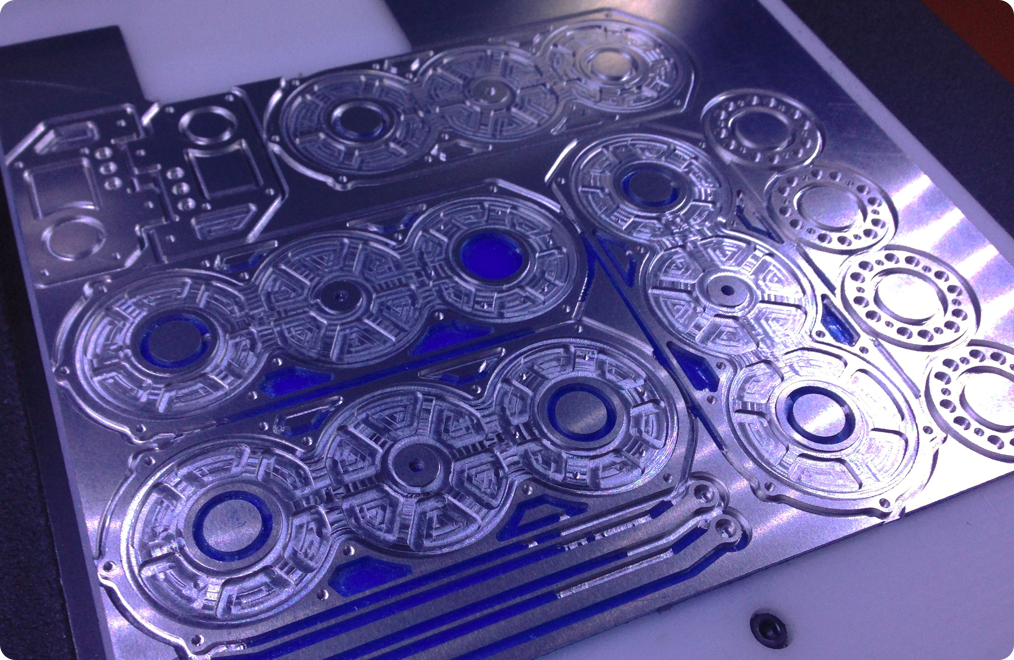
\includegraphics[width=0.45\textwidth]{CNC_milling_parts.png}
    \caption{CNC-ed parts} \label{fig:cnc}
\end{figure}

\section{Application}
\subsection{Set-up and Break-Down}
\begin{itemize}
    \item Set-up
    \begin{enumerate}
        \item Power the robot up.
        \item Join the Wi-Fi router on the host PC.
        \item Plug a gamepad to the host PC.
        \item Launch the host application.
    \end{enumerate}
    \item Break-Down
    \begin{enumerate}
        \item Shut the host PC down.
        \item Power the robot off.
    \end{enumerate}
\end{itemize}

\subsection{Mission Strategy}
We have two very powerful motors.
Their speed and torque make it easier to go beyond objects.
We are going to control the robot carefully because our camera is mounted statically.

\subsection{Experiments}
We confirmed that the connections between the host PC and the robot is successfully established, and communicated smoothly.
Actuators are also worked.

Some test case verify software.
Both robot and controller program are tested.

\subsection{Application in the Field}
Our robot worked well in school.
It can climb up and down stairs and communicate beyond the distance about \SI{20}{\metre}.
And there was no significant delay.

It did not work perfectly in the competition.
Firstly, radio was heavily congested.
This was because we could use only specified channel.
In school, we can communicate on a channel which not in use.
So even many (about over 20) access points existed, our robot works well.
But in the competition, our radio is eliminated by other team because our router is small and powerless.

Secondly, it could not climb continuous ramps because base of the robot hit them.
It is difficult to control 4 flippers at the same time through the views captured by a camera.
After some practice, we could climb better but it is still hard.

Figure \ref{fig:robotAndField} shows our robot running on a field in the competition.
\begin{figure}[!t]
    \centering
    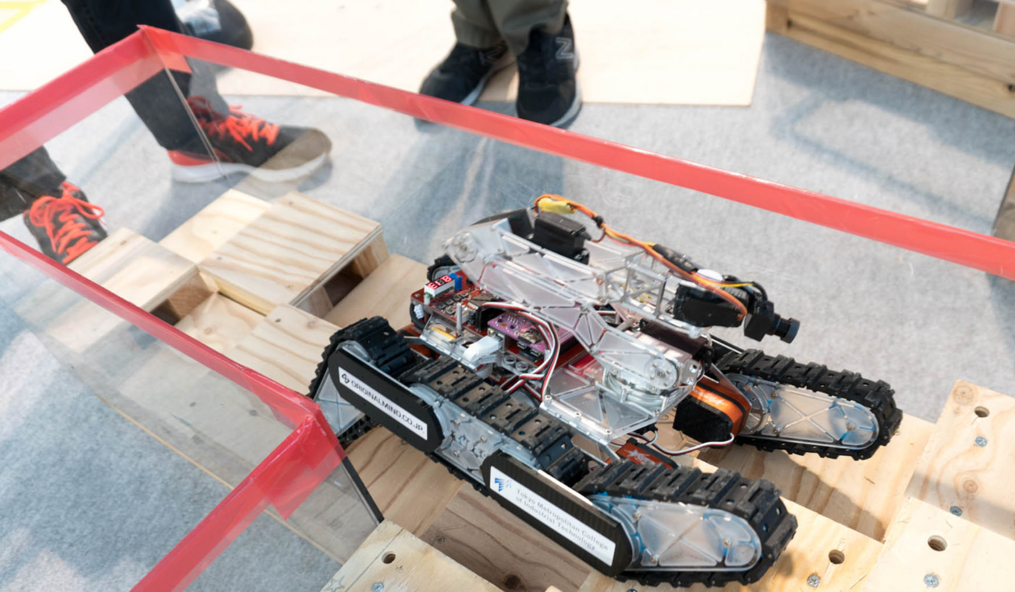
\includegraphics[width=0.45\textwidth]{robotAndField.png}
    \caption{Robot in the field} \label{fig:robotAndField}
\end{figure}

\section{Conclusion}
\subsection{What we learned so far}
\subsubsection{Mechanic}{}
We achieved building mini-version of conventional robots in RoboCup Rescue with flippers and arms.
It has mobility on roads with stairs and stones.
It also can run through more than half of given fields with operating over camera images, and it is possible to run on continuous fields like a big field.
The arms can be controlled remotely and complete pipestar.

We also found some problems.
Firstly, it is necessary to improve UI on software or make robot be able to detect its position because an operator cannot tell the direction of hardware over camera images.
Secondly, we gave up running on sand and falling because we had not made fields and practice.
Thirdly, sometimes the robot cannot commit spin turn because it is not fit in fields.
Finally, the robot does not have enough durability, especially crawlers.
Because of this, they often fall from pulleys, and we had to reset running.

\subsubsection{Electronic circuit}
Electrical circuit is also limited about size like mechanic.
To put all the components in limited space, we used many surface-mount devices.
It was very difficult to put motor drivers and a microcontroller on the same board.
Because motor drivers emit noises, and the microcontroller is very sensitive to them.
In addition, both of them emits lots of heat so we had to put them separately.
Large power lines for motor drivers also reduced the space.

\subsubsection{Software}
We learned network communications and image processing.
UDP broadcast packet was special for us since we only use HTTP requests daily.
It is also the first time for us to design an original protocol.

\subsection{What we are going to do}
Our robot is not equipped with any sensors to help an operator except a camera, so it is difficult to see what the situation it is in.
To solve this issue, we are planning to build a system that feedback many information by creating UI which indicates the situation with software like ROS.

\section{初心者向け}
\subsection{メカ}
\subsubsection{Size of Robot}
In order to clear the Centor Test, the size of the Robot shuld be within \SI{25}{\cm} squares.
Actually, the Robot can be cleard the Center Test even if the length of Robot is longer than 25cm.
As reference, the length of our Robot is approximately \SI{30}{\cm}, and it can clear the Center Test without problem line a stuck.
There is no restriction on the height of the competition field, so you shuld not pay an attention to the Robot's height. But if the height of the ZMP of Robot moves to high position, the stability of the Robot will become worse.

\subsubsection{Licomotion strategy}
不整地走行を行うロボットに用いられる移動方法は、主に車輪を用いる方法と、履帯を用いる方法がある。
There are several movement method used for Robot performing rough terrain travel.
車輪を用いる方法は、ハードウェア開発のリソースが非常に小さく、故にオープンソースとの親和性も非常に高いが、
ロボットと床との接地面積は履帯と比べて非常に小さいため、斜面などの強いグリップが必要なケースには向かない。
一方で、履帯はハードウェア開発のコストが非常に高いが、ロボットと床との接地面積は車輪に比べて非常に大きい。

もしもロボットが不整地の斜面を安定して登る必要があるのであれば、ロボットの移動手段には履帯を使うべきである。
移動手段に車輪を使った場合は、床との摩擦が足りず、斜面で安定して姿勢を制御することができない。
また、RMRC競技においては、履帯の方がAlign testを容易にクリア可能である。

\subsubsection{Flipper arm}
ロボットにFlipper armを搭載する事は、ロボットの車輪の半径(履帯の場合はスプロケットの半径)よりも大きな段差を乗り越えることを可能にする。
ロボットの前方のみにFlipper armを取り付けるだけでは、Hurdles testをクリアする事は困難である。
ロボットの後方にもFlipper armを取り付け、ロボットのボディを持ち上げる機構を実現することで、この問題は解決できる。

\subsubsection{Productivity}
ロボットのパーツの製造には、積極的に3D Printerを使用するべきである。
多くの人が真似できるハードウェアは、オープンソースへの貢献度が高い。
また、なるべくチープな3D Printerでも製造可能なように、パーツの要求精度がそう高くならないような設計をするのも重要である。
また、配線作業においては、特殊な配線をなるべく必要としない、Connector to Connector結線のみで構成されたシステムが好ましい。

\subsection{電気}
\begin{itemize}
    \item We do not recommend beginners to use GR-Peach.
    You should use more powerful MCU like Raspberry PI.
    GR-Peach can handle the situation only if it is programmed to use hardware resources effectively.
    This makes you have to write lots of codes since it is not famous and there is a few resources on the Internet.
    With more famous boards like Raspberry PI, you can reuse resources and you do not have to worry about latency.
    \item VNH5019 is not powerful enough to drive motors.
    Our motor driver was broken on the final day of the competition.
    It is surface-mounted IC, so replacement was not easy.
    You should use more powerful and replaceable IC like Pololu 18v25.
    \item If you use \SI{5}{\V} or \SI{3.3}{\V} devices, you should produce the voltage by DC-DC converters rather than switching regulators.
    Switching regulator wastes energy to drop voltage.
    This makes it hotter and limit the amount of current.
    So you might get some problems like voltage spike.
    DC-DC converters can produce constant voltage more efficient way.
    Although DC-DC converters require more components than switching regulators, it is much better to use DC-DC converters.
\end{itemize}

\subsection{ソフトウェア}
\begin{itemize}
    \item Again, you should not use GR-Peach.
    It is mbed-enabled and you can write a program with mbed library.
    But it is much easier to use complete programs provided by big community.
    You can stream video images by connecting a camera and run a built-in program with Raspberry PI for example.
    You should not waste time to basic activities.
    You should spent more time to more important tasks like OpenCV.
    \item I encourage you to use AOP(Aspect Oriented Programming) technique.
    It makes your code more independent.
    AOP will give you the new sight of programming.
\end{itemize}

\appendices

\section{Team members and Their Contributions}
\begin{itemize}
    \item Yuichi Kikuchi \hfill Mechanical design
    \item Takumi Komori \hfill Electronic circuit and software design
\end{itemize}

\begin{table*}
    \renewcommand{\arraystretch}{1}
    \tabcolsep=0.1cm
    \caption{Robot Specification}
    \label{tab:SystemOp1}
    \centering
    \begin{tabular}{|l|r|}
    \hline
    Attribute & Value \\ \hline
    Name & TUPAC \\
    Robot Weight & \SI{3.5}{\kg} \\
    Weight including transportation case & \SI{3.6}{\kg} \\
    Transportation size & W:0.24 x L:0.32 x H:\SI{0.20}{\m} \\
    Typical operation size & W:0.22 x L:0.44 x H:\SI{0.15}{\m} \\
    Unpack and assembly time & 1 min \\
    Startup time (off to full operation) & \SI{3}{\min} \\
    Power consumption (idle/ typical/ max) & 20 / 60 / \SI{200}{\W} \\
    Battery endurance (idle/ normal/ heavy load) & 60 / 20 / \SI{10}{\min}\\
    Any other interesting attribute & Audio playback function\\
    Cost & 1091.24 USD \\
    \hline
    \end{tabular}
\end{table*}
\begin{table*}
% increase table row spacing, adjust to taste
\renewcommand{\arraystretch}{1}
 \tabcolsep=0.1cm
\caption{Hardware Components List} \label{tbl:hardware_list}
\centering
\begin{tabular}{|c|c|c|c|}
\hline
Part & Brand \& Model & Unit Price & Num. \\ \hline
Drive motors + gears & \href{http://store.shopping.yahoo.co.jp/suzakulab/rs-380phgm019.html}{RS-380PH + IG32 1/19} & JPY 4273 & 2 \\ 
Servo motors for Flipper & RoboStar SBRS-5314HTG & JPY 4329 & 4 \\
Servo motors for Robot arm & KONDO KRS-2346ICS & JPY 16740 & 3 \\
Servo motors for Manipulation & JR-PROPO DSR3801 & JPY 11000 & 2 \\ \hline
\multirow{3}{*}{Constructional material} & Polycarbonate plate t4 220x300 & JPY 450 & 5 \\
& A2017 plate t2 220x300 & JPY 1000 & 1 \\
& A5052 plate t1.5 220x300 & JPY 1000 & 1 \\ \hline
DC-DC Converter & \href{http://power.murata.com/en/okl-t-6-w12n-c.html}{OKL-T/6-W12N-C} & JPY 600 & 1 \\
Batteries & \href{http://www.kypom.com/pro_detail.asp?id=763}{KT2200/35-2S} & JPY 1764 & 1 \\
Motor drivers & \href{https://www.pololu.com/product/1449}{Pololu VNH 5019A} & USD 10.95 & 2 \\
Microcontroller & \href{https://developer.mbed.org/platforms/Renesas-GR-PEACH/}{GR-Peach} & JPY 8940 & 1 \\
WiFi Router & \href{http://www2.elecom.co.jp/products/WRH-583RD2-S.html}{WRH-583RD2-S} & JPY 3472 & 1 \\
Camera module & NTSC FPV-Camera for Drone & JPY 1790 & 1 \\ \hline
Rugged Operator Laptop & \href{http://www.apple.com}{MacBook} & - & 1 \\
\hline 
\end{tabular}
\end{table*}
\begin{table*}
% increase table row spacing, adjust to taste
\renewcommand{\arraystretch}{1}
 \tabcolsep=0.1cm

\caption{Software List}
\label{tbl:software_list}
\centering
\begin{tabular}{|c|c|c|c|}
\hline
Name & Version & License & Usage \\
\hline
 \href{https://www.mbed.com/en/}{mbed OS 5} & 133 & Apache 2.0 & Robot software \\
 \href{https://developer.mbed.org/teams/Renesas/code/GR-PEACH_video/}{GR-PEACH\_video} & 16/6/30 & \href{https://os.mbed.com/teams/Renesas/wiki/About-LICENSE}{Renesas} & Video Processing \\
 \href{https://developer.mbed.org/teams/Renesas/code/GraphicsFramework/}{GraphicsFramework} & 16/12/14 & \href{https://os.mbed.com/teams/Renesas/wiki/About-LICENSE}{Renesas} & JCU \\
 \href{https://developer.mbed.org/teams/Renesas/code/R_BSP/}{R\_BSP} & 16/5/31 & \href{https://os.mbed.com/teams/Renesas/wiki/About-LICENSE}{Renesas} & \(\mathrm{I^2S}\) \\
 \href{https://github.com/Daij-Djan/DDHidLib}{DDHidLib} & 1.1.1 & MIT & Gamepad control \\
 \href{https://github.com/360Controller/360Controller}{360Controller} & 0.16.4 & GPL 2.0 & Gamepad driver \\
 \href{https://github.com/robbiehanson/CocoaAsyncSocket}{CocoaAsyncSocket} & 7.6.0 & open & UDP communication \\
 \href{https://github.com/CocoaPods/CocoaPods}{CocoaPods} & 1.3.1 & MIT & Library Management \\
 \href{https://github.com/steipete/Aspects}{Aspects} & 1.4.2 & MIT & AOP \\
 \href{http://zbar.sourceforge.net}{ZBar} & 0.10 & LGPL 2.1 & QR code detection \\
 \href{http://opencv.org}{OpenCV} & 3.2.0 & BSD & Image processing \\
\hline
\end{tabular}
\end{table*}

\section{CAD Drawings}
Figure \ref{fig:hardware} shows the drawing of the hardware.
Figure \ref{fig:main_3d} shows the 3D model of the main board.
\begin{figure*}[!p]
    \centering
    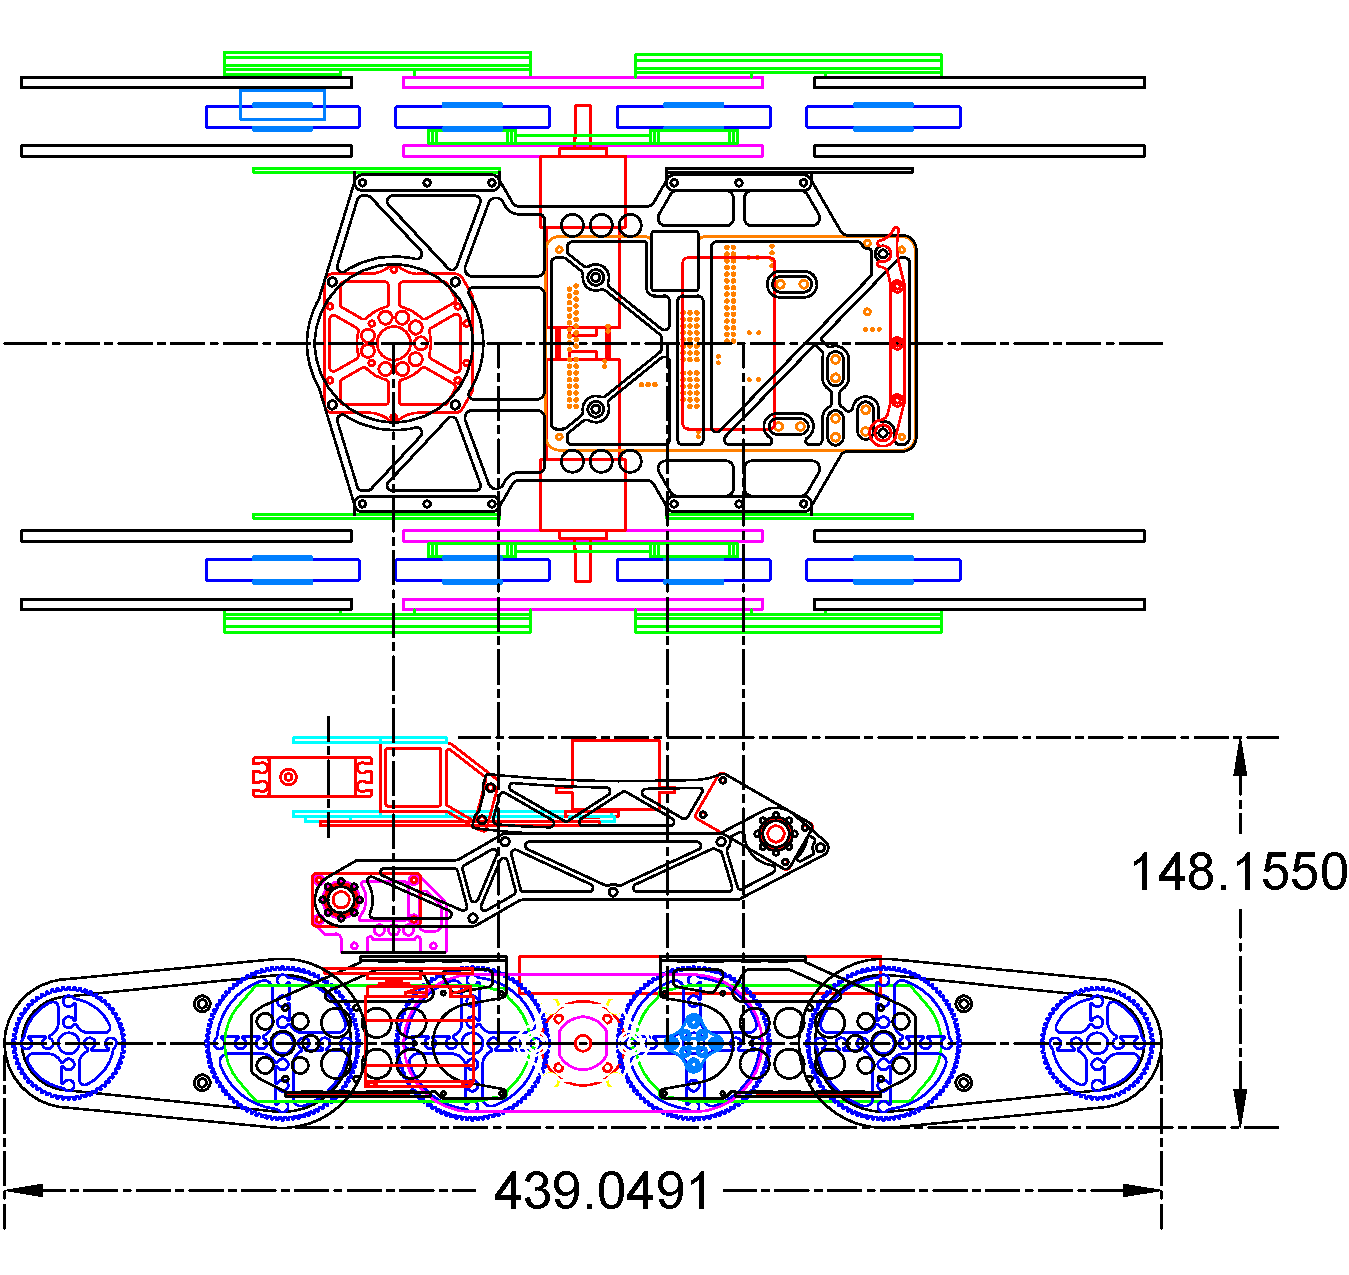
\includegraphics[width=1.0\textwidth]{CAD.pdf}
    \caption{Hardware CAD drawing} \label{fig:hardware}
\end{figure*}
\begin{figure*}[!p]
    \centering
    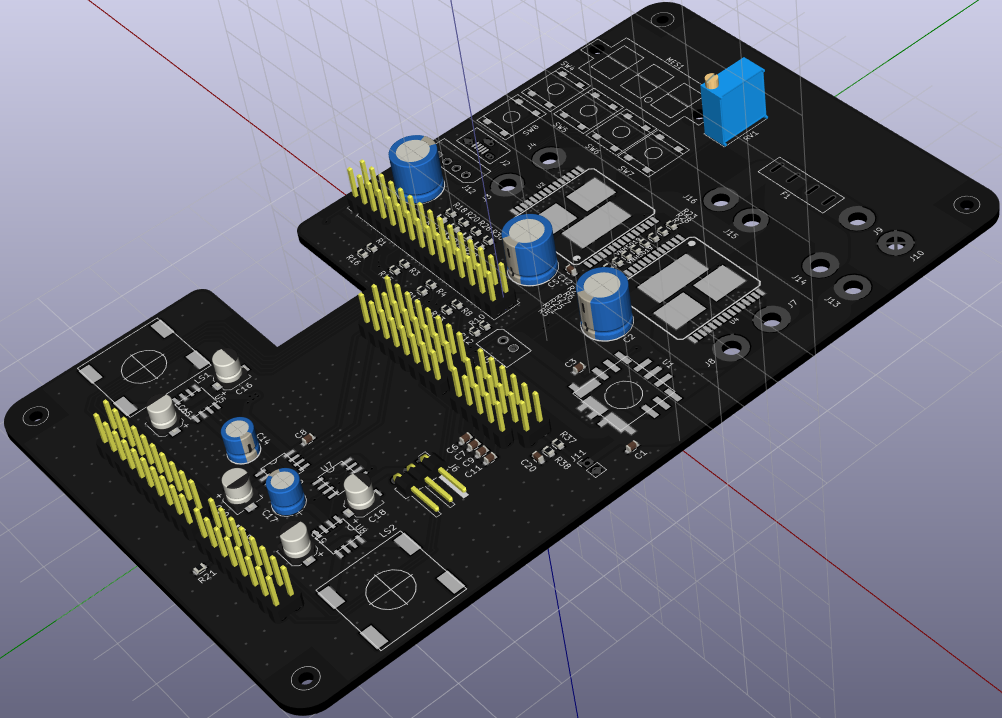
\includegraphics[width=1.0\textwidth]{main.png}
    \caption{Electronic circuit board 3D model} \label{fig:main_3d}
\end{figure*}

\section{Lists}
See Table \ref{tab:SystemOp1} for the systems list.
\subsection{Systems List}

\subsection{Hardware Components List}
See Table \ref{tbl:hardware_list} for the hardware components list.

\subsection{Software List}
See Table \ref{tbl:software_list} for the software list.

\section*{Acknowledgment}
The authors would like to thank our mother and father, Kazutoshi Tominaga for advising us, Yusuke Tada for milling our hardware, Naomi Chikuma and Masayuki Okugawa for helping our participation, and Renesas Electronics for helping us with GR-Peach. %, and Tupac Shakur for sparking our brains.

\end{document}
